\section{Event mentions and two temporal layers}
\label{sec:events}

Event reconstruction accepts already typed mentions containing a predicate,
actor and object identifiers, place, evidence references, and temporal metadata.
It does not extract events autonomously from reports, posts, or video. This
boundary differs from supervised span-based extraction, where predicted triggers
and arguments are evaluated against annotated text
\citep{wadden2019dygiepp}. The implemented contribution is conservative
organization of supplied assertions.

Communication mentions use publication timestamps; physical mentions require
supplied earliest and latest event-time bounds to enter their timeline. Missing
or partially bounded physical time is preserved without substituting publication
time. Figure~\ref{fig:dual} presents the two layers. Pairwise interval comparisons
produce before, after, overlap, or unknown relations, with every temporal edge
explicitly marked noncausal. Ordering reports cannot establish that one physical
action caused another.

\begin{figure}[tb]
\centering
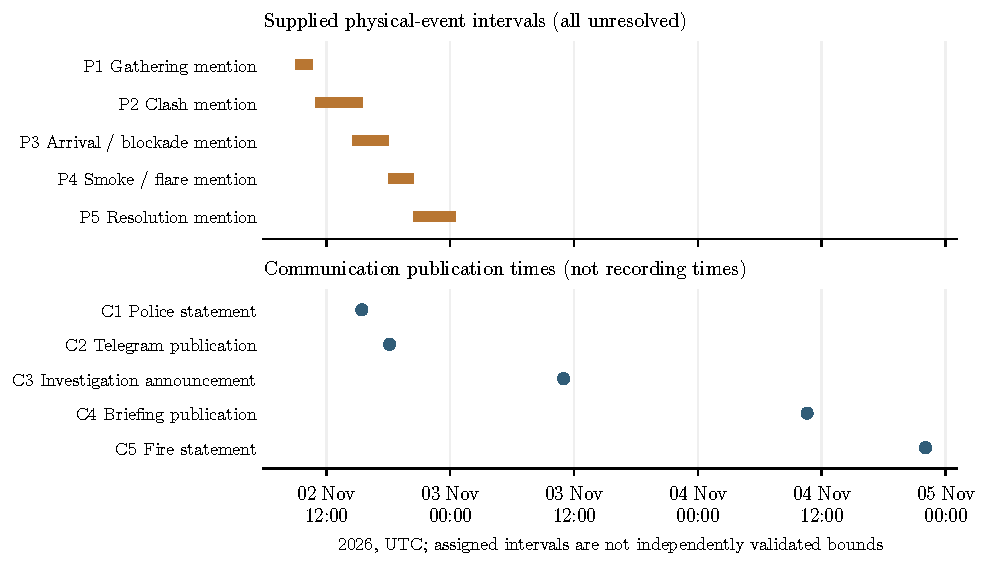
\includegraphics[width=\linewidth]{dual_timeline.pdf}
\caption{Separate communication and physical-event timelines. Publication times
locate communications; analyst-supplied intervals locate reported physical
episodes. Overlapping bounds and unresolved mentions remain visible, and temporal
order carries no causal interpretation.}
\label{fig:dual}
\end{figure}

Exact agreement of normalized predicate, actor identifiers, object identifiers,
and place can produce a reviewable possible-same link, subject to temporal
compatibility and supplied cannot-link constraints. The function never merges
mentions. This restraint matters because similar descriptions can refer to
different event instances, a difficulty emphasized by ECB+
\citep{cybulska2014ecbplus}. Cannot-link constraints preserve analyst-specified
distinctions; they are not independently discovered identity judgments.

The curated timeline contains five physical and five communication mentions.
All ten remain unresolved, with zero possible-same links. Actors, intervals,
participant positions, and qualitative evidence tiers are supplied in the
builder's literal input list. Those tiers describe the asserted evidence basis,
not calibrated confidence or verified physical occurrence. Thus the artifact
demonstrates reproducible temporal organization and explicit uncertainty; its
counts do not measure event-discovery recall or reconstruction accuracy.
